\documentclass[12pt, a4paper, oneside]{ctexart}
\usepackage{amsmath,caption, amsthm, amssymb, bm, graphicx, hyperref, mathrsfs,subfig,cite}

\title{Assignment1 Environment}
\author{PhilFan 樊铧纬}
\date{\today}
\linespread{1.5}
\newcounter{problemname}
\newenvironment{problem}{\stepcounter{problemname}\par\noindent\textbf{题目\arabic{problemname}. }}{\\\par}
\newenvironment{solution}{\par\noindent\textbf{解答. }}{\\\par}
\newenvironment{note}{\par\noindent\textbf{题目\arabic{problemname}的注记. }}{\\\par}


\begin{document}
\maketitle
在CC98开了一个记录的楼,记录学习中遇到的问题和学习过程;~\cite{ref1}
\begin{problem}
	1. 创建你的gitee帐号,创建一个叫math-soft的源,将其设成公开仓库\\
	2. 在你的源内,增加一篇文档,名为:enviroment.tex,内容为对你参加课程学习的计算环境的描述,要求至少包含\\
		你的计算机型号,CPU型号,内存大小,硬盘大小,显卡型号 (指你真正的计算机\\
		你的Linux实现方式。如果是虚拟机,描述一下虚拟机的内存大小和硬盘大小\\
		你的Linux版本,和安装了哪些额外的软件(系统自带的不用列,自己安装的不论是否是我视频中有的尽量列出\\
		你的编辑器和你的gcc编译器的版本\\
		用最多不超过200字评估一下你在未来的学习和工作中使用Linux环境工作的可能性和可能场景\\
		文章应该能用latex编译通过可以参考我的文件,注意字体需要安装\\
\end{problem}

\begin{solution}
	\setcounter{section}{1}
	\subsection{计算机}
		\paragraph{计算机型号}Huawei MateBook 13
		\paragraph{CPU}AMD Ryzen 5 4600H with Radeon Graphic 3.00 GHz
		\paragraph{内存}16GB			
		\paragraph{硬盘大小}476GB
		\paragraph{显卡}无独立显卡,为集成显卡
	\subsection{Linux}
		\paragraph{实现方式}虚拟机VMware Workstation 16 Player\\
		\paragraph{虚拟机内存}
		使用fdisk查询\\
	\begin{tabular}{cccc}
		\hline
		name&total&used&free\\
		内存&3.8Gi&1.2Gi&928M\\
		交换&2.1Gi&62Mi&2.0Gi\\
		\hline
	\end{tabular}
		\paragraph{虚拟机磁盘}
		磁盘数据\\
\begin{tabular}{cccccc}
	\hline
	文件系统& 大小& 已用&  可用& 已用& 挂载点\\
	tmpfs&392M&2.0M&390M&1&/run\\
	sda3&34G&26G&6.7G&80&/\\
	tmpf&2.0G&0&2.0G&0&/dev/shm\\
	tmpfs&5.0M&4.0K&5.0M&1&/run/lock\\
	/dev/sda2&512M&6.1M&506M&2&/boot/efi\\
	tmpfs&392M&112K&392M&1&/run/user/1000\\
	/dev/sr1&3.6G& 3.6G&0&100&/media/philfan/Ubuntu 22.04.1 LTS amd64\\
	/dev/sr0&127M&127M&0&100&/media/philfan/CDROM\\
	\hline
\end{tabular}
	\subsection{software}
		\paragraph{Linux}
			版本Ubuntu 22.04.1 LTS amd64
		\paragraph{listofsoftware}
			方法:apt list /-/-installed\\
			所有软件的列表放在./software.txt下,因为太长了\\

			使用gpt优化答案\\
		%	"comm -23 <(apt list --installed | cut -d '/' -f 1 | sort) <(gzip -dc /var/log/installer/initial-status.gz | sed -n 's/^Package: //p' | sort) > installed_packages.txt"\\

		%\input{software.txt}


	\subsection{compiler}
		\paragraph{编辑器}
			Vim\\
		\paragraph{gcc}
			gcc version 11.3.0 (Ubuntu 11.3.0-1ubuntu1~22.04.1)\\
		
	\subsection{application}
		\paragraph{课程需要}
	嵌入式、机器人实践(ROS)等课程可能会用到linux环境;\\
	讲到的编辑器vim、makefile、latex工具等也可以极大提高我的工作效率。\\
		\paragraph{兴趣}
			对树梅派比较感兴趣,希望学习一些linux环境,进而掌握如服务器开发、脚本编写等小项目的撰写。\\
		\paragraph{感受}
			双手脱离鼠标操作电脑难道不是世界上最酷的事情吗doge\\
\end{solution}

\begin{problem}
	上课例子程序展示
\end{problem}

\begin{solution}
	相关操作文件放在了../lec1下的文件夹下\\
	\setcounter{section}{1}
	
	\subsection{deal-ii-step57}
		图\ref{img} 显示了deal-ii 例子中流线的情况抗

		记得要点击solve\\
		\begin{figure}
			\centering
			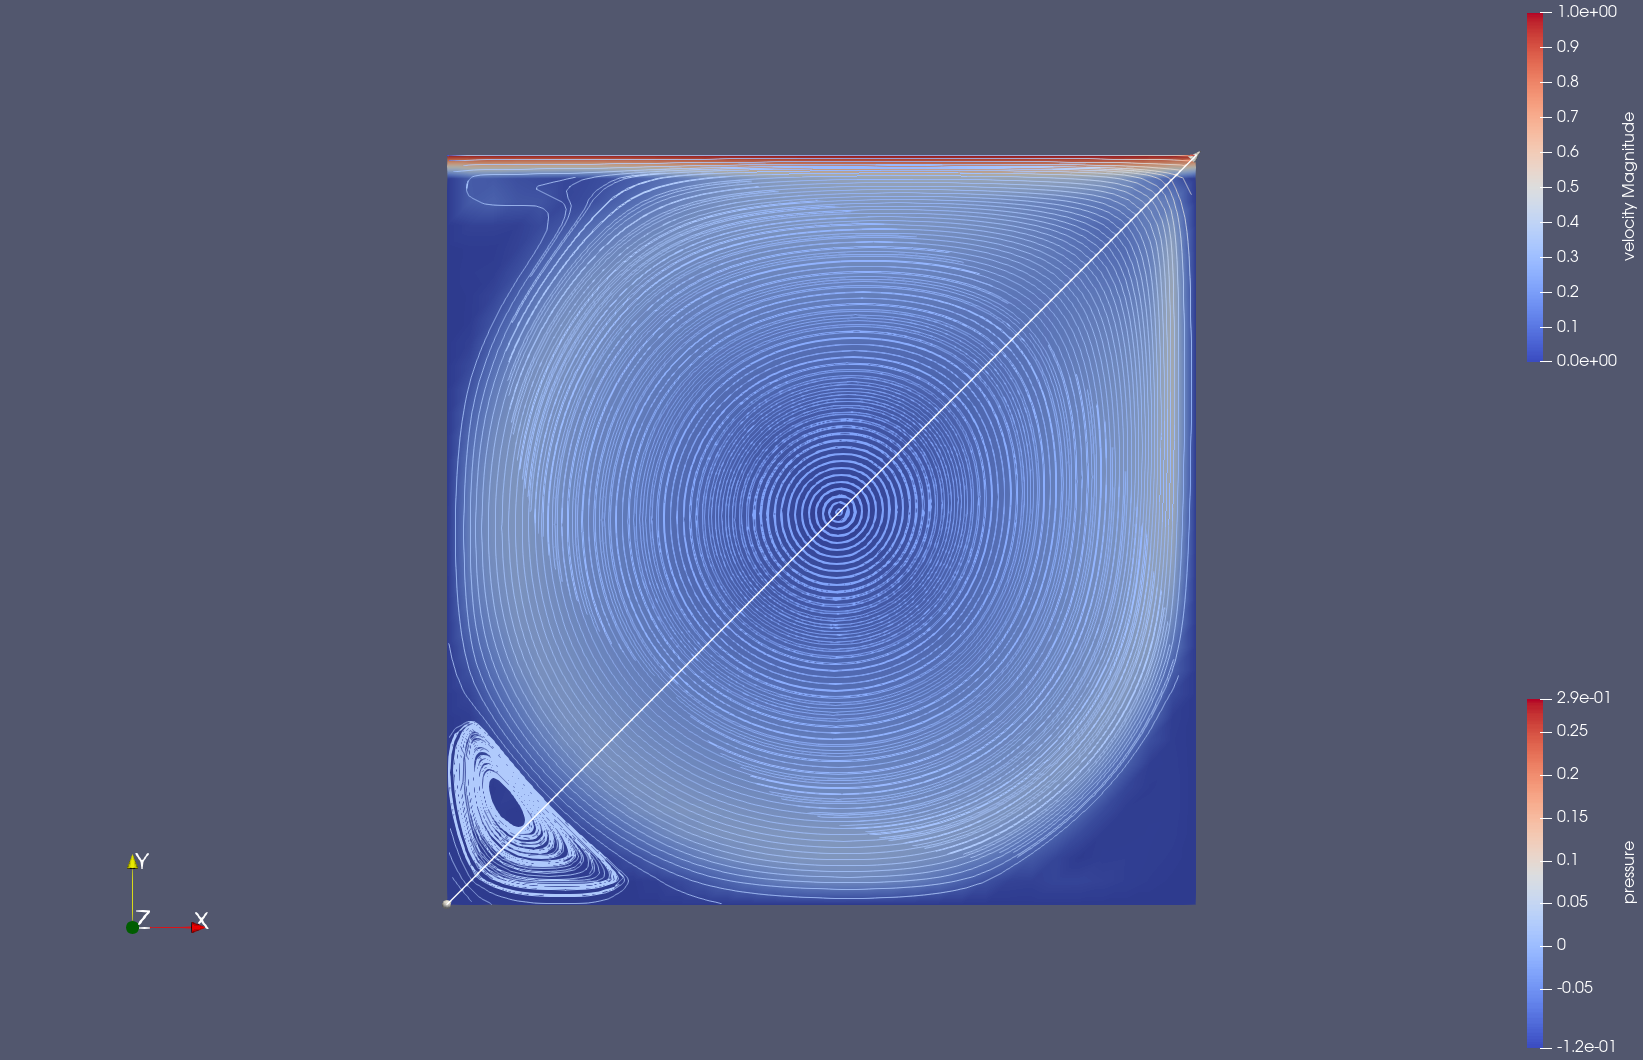
\includegraphics[width=.8\textwidth]{pic.png} %1.png是图片文件的相对路径
			\caption{pic} %caption是图片的标题
			\label{img} %此处的label相当于一个图片的专属标志,目的是方便上下文的引用
		\end{figure}\\
\end{solution}


% 使用 BibTeX 管理文献引用
\bibliographystyle{plain}
\bibliography{references}

\end{document}


